\documentclass[8pt]{beamer}

\usetheme{metropolis}
\usepackage{appendixnumberbeamer}
\usepackage{xcolor}
\usepackage{booktabs}
\usepackage[scale=2]{ccicons}
\usepackage{graphicx}
\usepackage{pgfplots}
\usepgfplotslibrary{dateplot}
\usepackage{caption}
\usepackage{subcaption}
\usepackage{xspace}
\usepackage{hyperref,xcolor}
\usepackage{textpos}
\usepackage{appendixnumberbeamer}
\usepackage{makeidx}
\usepackage{verbatim}
\usepackage{tikz}
\usepackage{xcolor}

\usepackage{listings}
\usepackage{tikz}
\usetikzlibrary{arrows.meta}
\usetikzlibrary{positioning}
\definecolor{winered}{rgb}{0.5,0,0}
\newcommand{\themename}{\textbf{\textsc{metropolis}}\xspace}
\lstset{
	numbers=left,               % Ort der Zeilennummern
	stepnumber=2,               % Abstand zwischen den Zeilennummern       
	numberfirstline=false,
	basicstyle=\ttfamily,
	columns=fullflexible,
	frame=single,
	breaklines=true,
	postbreak=\mbox{\textcolor{red}{$\hookrightarrow$}\space},
	showstringspaces=false
}


\defbeamertemplate*{background canvas}{bg}
{%
	\color{white}\vrule width\paperwidth height\paperheight% added bg color
}

\definecolor{OliveGreen}{rgb}{0,0.5,0}



\title{Systematic Studies On Track Reconstruction Efficiency At Belle II}
%\subtitle{A modern beamer theme}
\date{00.01.2020}
\author{Martin Sobotzik (msobotzi@students.uni-mainz.de)}
\institute{Johannes Gutenberg-Universit\"at Mainz}
% \titlegraphic{\hfill\includegraphics[height=1.5cm]{logo.pdf}}

\definecolor{darkblue}{rgb}{0,0,.5}
\hypersetup{pdftex=true, colorlinks=true, breaklinks=true, linkcolor=darkblue, menucolor=darkblue, pagecolor=darkblue, urlcolor=darkblue}


%citecolor={winered} %Gives errors when turned on
%allcolors={winered} %Gives errors when turned on

\begin{document}
\maketitle
%
\setbeamertemplate{frame footer}{}

%\section{Reproducing Plots}



\begin{frame}{Outline}




	\begin{itemize}
		\item Overview on the Belle II experiment
		\item Bhabha kinematics at Belle II
		\item Preparation for calculating the tracking efficiency
		\item Phase2 tracking efficiency
		\item Phase3 tracking efficiency
		\item Comparing phase2 with phase3
		\item Conclusion
		
		
	\end{itemize}
\end{frame}



\begin{frame}{Motivation}
	\begin{itemize}
		\item At an electron-positron accelerator most outgoing particles are again electrons and positrons (these events are called Bhabha events)
		\item These events can be used to estimate the performance of the tracking detectors
		\item If the \textit{tag} particle in a Bhabha event has a track than the \textit{probe} particle also should have a track associated 
		
		$\rightarrow$ a tracking efficiency can be calculated
	\end{itemize}
\end{frame}


\section{Overview Of The Belle II Experiment}

\begin{frame}{Belle II Schedule And Luminosity Goals}

	\begin{textblock*}{7cm}(4.8cm,-2.8cm)
	\begin{figure}
		\includegraphics[width=7cm]{VBilder/Lumen}
	\end{figure}
	
	
\end{textblock*}






	
	\begin{textblock*}{5cm}(-0cm,-3cm)
		\begin{center}	
			\begin{itemize}
				\item Phase1: accelerator commissioning and background estimation (completed in 2016)
				\item Phase2: collision runs and background studies with partially installed detector (completed in 2018)
				\item Phase3: data taking with the whole detector (started in April 2019)
			\end{itemize}
		\end{center}
		
	\end{textblock*}
	

	
	
	
	
\end{frame}


\begin{frame}{The SuperKEKB $\textrm{e}^+\textrm{e}^-$ collider}



\begin{textblock*}{4.5cm}(-0cm,-3cm)
	\begin{center}	
		\begin{itemize}
			\item Asymmetric $B$-factory
			\item Center-of-mass close to $\Upsilon(4\textrm{S})$ $\sim 10.5\,\textrm{GeV}$
			\item Upgrade of the KEKB collider:
			\begin{itemize}
				\item Larger beam current
				\item Reduced beam size
			\end{itemize}
		
		
		\item<3> $\rightarrow$ Luminosity increase x40
		\item<3> Designed peak luminosity of $8\cdot 10^{35}\,\textrm{cm}^{-2}\textrm{s}^{-1}$
		\item<3> Planned data sample corresponding to a recorded integrated luminosity of $\sim 50\,\textrm{ab}^{-1}$
		
		
		\end{itemize}
	\end{center}
	
\end{textblock*}


\begin{textblock*}{7cm}(4.8cm,-3cm)
	\begin{figure}
		\includegraphics[width=6.5cm]{VBilder/SuperKEKB}
	\end{figure}
	
	
\end{textblock*}

\begin{textblock*}{7cm}(-0.8cm,0cm)
	\begin{figure}
		\includegraphics<2>[width=7cm]{VBilder/Beamsize.pdf}
	\end{figure}
	
	
\end{textblock*}




\end{frame}


\begin{frame}{The Belle II Detector}

\begin{figure}
	\includegraphics[width=\textwidth]{VBilder/Belle2.pdf}
\end{figure}


	
\end{frame}

\begin{frame}{Vertex Detectors}
	
	
		\begin{textblock*}{10cm}(2cm,-1.9cm)
		\begin{figure}
			\includegraphics[width=6cm]{VBilder/PXD_SVD}
		\end{figure}
		
		
	\end{textblock*}
	
	
	\begin{textblock*}{10cm}(-0cm,-3.7cm)
		Vertex Detectors:		
			\begin{itemize}
				\item Consists of Pixel Detector (PXD) and Silicon Vertex Detector (SVD)
				\item Both detectors consist of multiple ladders of strip detectors
				\item During phase2, only a fraction of the VXD detectors were installed
				\item During phase3, the complete SVD and roughly half of the PXD were installed
				\item Acceptance: $17.0^{\circ} < \theta < 150.0^{\circ}$ 
			\end{itemize}
		



	\end{textblock*}
	
	

	
	
	
\end{frame}


\begin{frame}{Central Drift Chamber}

	\begin{textblock*}{4cm}(7cm,-2.5cm)
		\begin{figure}
			Axial
			\includegraphics[width=\textwidth]{VBilder/axial}
		\end{figure}
	\end{textblock*}

	\begin{textblock*}{4cm}(7cm,-1.25cm)
		
		\begin{figure}
			Stereo
			\includegraphics[width=\textwidth]{VBilder/stereo}
		\end{figure}
	\end{textblock*}




	\begin{textblock*}{10cm}(0cm,-3.7cm)
	
		Central Drift Chamber:
		\begin{itemize}
			\item Consists of 14336 sense wires arranged in 56 layers
			\item 6 layers are combined to a superlayer (with an exception to innermost superlayer)
			\item There are 5 axial and 4 stereo superlayers
			\item The electric field is provided by 42240 field wires
			\item Charged particles ionize the gas. 
			
			The signal is then read out by the sense wires  
			\item Acceptance: $17.0^{\circ} < \theta < 150.0^{\circ}$ 
		\end{itemize}

	\end{textblock*}


\begin{textblock*}{10cm}(0cm,1cm)
	\includegraphics[width=\textwidth]{VBilder/cdc}
\end{textblock*}


\end{frame}


\begin{frame}{Electromagnetic Calorimeter}
	\begin{textblock*}{6cm}(5.5cm,-3.cm)
		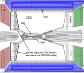
\includegraphics[width=\textwidth]{VBilder/ecl2}
	\end{textblock*}

\begin{textblock*}{5.2cm}(0cm,-3.7cm)
	Electromagnetic Calorimeter:
	\begin{itemize}
		\item Consists of 8936 CsI(Tl) crystals
		\item Separation in \textcolor{blue}{barrel}, \textcolor{OliveGreen}{forward end cap} and \textcolor{red}{backward end cap}
		\item There are two $\sim 1^{\circ}$ wide gaps at transition between the regions
		\item Main tasks:
		\begin{itemize}
			\item High efficiency photon detection, plus determination of their energy and angular coordinates
			\item Electron identification
			\item Generation of a proper signal for the trigger
		\end{itemize}
		\item Acceptance: $12.4^{\circ} < \theta < 155.1^{\circ}$ 
	\end{itemize}
\end{textblock*}


\end{frame}

\section{Bhabha Kinematics At Belle II}

\begin{frame}{Bhabha Kinematics At Belle II}
	
	
	

	
	\begin{textblock*}{5.5cm}(6cm,0.cm)
		
		\includegraphics[width=\textwidth]{VBilder/theta_lab}
	\end{textblock*}

	\begin{textblock*}{5.5cm}(0cm,0.0cm)
	
	\includegraphics[width=\textwidth]{VBilder/ee}
\end{textblock*}


	\begin{textblock*}{5cm}(6cm,-3.cm)
		\begin{itemize}
			\item The beams have asymmetric energies
			\item The beams are hitting each other under an angle of $1.26^{\circ}$
		\end{itemize}
	\end{textblock*}

\begin{textblock*}{5.5cm}(-0.5cm,-3.7cm)
	
	\includegraphics[width=\textwidth]{VBilder/finalCross}
\end{textblock*}




%\begin{textblock*}{2cm}(4.7cm,1.8cm)

%	\begin{tikzpicture}
%		\draw[-{Triangle[width=18pt,length=8pt]}, line width=10pt](0,0) -- (1, 0);
%	\end{tikzpicture}
%	\centering
%	Boost
%\end{textblock*}
	
	


\end{frame}





\section{Preparation For Calculating The Tracking Efficiency}


\begin{frame}{Reconstruction Bhabha Events With Basf2}

\lstset{language=Python}
\lstset{label={lst:code_direct}}
\lstset{basicstyle=\scriptsize}

\begin{textblock*}{\textwidth}(-0cm,-3.7cm)

\lstinputlisting[language=Python]{mesh.py}


\end{textblock*}

\begin{textblock*}{11cm}(0cm,0cm)
			
\begin{figure}[h!]
	\centering
	\begin{minipage}[b]{0.45\linewidth}
		\centering
		\includegraphics[width=\textwidth]{VBilder/nCandAll.pdf}
	\end{minipage}
	\hspace{0.5cm}
	\begin{minipage}[b]{0.45\linewidth}
		\centering
		\includegraphics[width=\textwidth]{VBilder/Mall.pdf}
	\end{minipage}
	
\end{figure}


\end{textblock*}

\begin{textblock*}{11cm}(0cm,0.3cm)
	\centering
	Single phase2 MC10 Bhabha file
\end{textblock*}

\begin{textblock*}{4cm}(2.8cm,1.3cm)
	24100 Events
\end{textblock*}

\begin{textblock*}{4cm}(7.8cm,1.3cm)
	417899 Candidates
\end{textblock*}



\end{frame}


\begin{frame}{Introducing Cuts}
	\begin{textblock*}{11cm}(0cm,-3.7cm)
	\begin{itemize}
		\item $8\,\textrm{GeV} < \textrm{M} < 12\,\textrm{GeV}$
		\item Exactly 2 clusters with at least $3.5\,\textrm{GeV}$ per event and one cluster has to have at least $4.5\,\textrm{GeV}$
		\item Number of reconstructed tracks per event $< 7$
		\item Total energy in the ECL $< 15\,\textrm{GeV}$
	\end{itemize}

\end{textblock*}

\begin{textblock*}{11cm}(0cm,0cm)
\begin{figure}[h!]
	\centering
	\begin{minipage}[b]{0.45\linewidth}
		\centering
		\includegraphics[width=\textwidth]{VBilder/nCandNoMCInfo.pdf}
	\end{minipage}
	\hspace{0.5cm}
	\pause[2]
	\begin{minipage}[b]{0.45\linewidth}
		\centering
		\includegraphics[width=\textwidth]{VBilder/nCandData.pdf}
	\end{minipage}
	
\end{figure}

\end{textblock*}
\pause[1]

\begin{textblock*}{5cm}(0.1cm,0.3cm)
	\centering
	Single phase2 MC10 Bhabha file
\end{textblock*}


\begin{textblock*}{4cm}(2.8cm,1.3cm)
	14581 Events
\end{textblock*}
\pause[2]

\begin{textblock*}{4cm}(8.5cm,1.3cm)
	41853 Events
\end{textblock*}


\begin{textblock*}{4cm}(7.cm,0.3cm)
	Single phase2 data file
\end{textblock*}


\pause[3]

\begin{textblock*}{5cm}(3.2cm,-0.5cm)
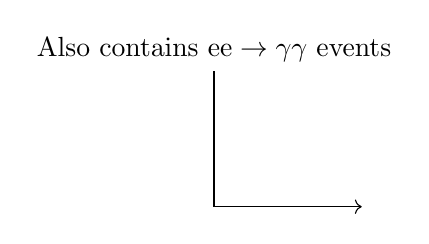
\begin{tikzpicture}[node distance=3cm]

% nodes
\node (A) at (3, 0) {};
\node (B) at (1, 2) {Also contains $\textrm{ee}\rightarrow\gamma \gamma$ events};
\draw[<-, to path={-| (\tikztotarget)}]
(A) edge (B);

\end{tikzpicture}


\end{textblock*}
\end{frame}



\begin{frame}{Bhabha Event Selection}
	
	\begin{figure}
		\centering
		\includegraphics<1>[width=\textwidth]{Plots/b2b_2}
	\end{figure}
	
\end{frame}

\begin{frame}{Bhabha Event Selection}
	
	\begin{textblock*}{0.5\textwidth}(0cm,-3cm)
		\centering
		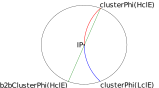
\includegraphics[width=4.5cm]{VBilder/b2b_2}
	\end{textblock*}
	
	\begin{textblock*}{0.5\textwidth}(5.5cm,-3cm)
		\centering
		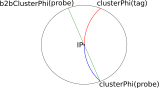
\includegraphics[width=4.5cm]{VBilder/b2b_3}
	\end{textblock*}
	
	
	\begin{textblock*}{1\textwidth}(0cm,0.cm)
		\centering
		\includegraphics[width=\textwidth]{VBilder/sb2b_Data.pdf}
	\end{textblock*}
	
	
\pause	
	
		\begin{textblock*}{1\textwidth}(0cm,0.cm)
		\centering
		\includegraphics[width=\textwidth]{VBilder/sb2b_MC.pdf}
	\end{textblock*}
	
	

	
\end{frame}


\begin{frame}{Trigger}
	
	\begin{textblock*}{6.5cm}(5.5cm,-0.2cm)
		\includegraphics[width=\textwidth]{VBilder/DataTrigger}
	\end{textblock*}
	
	
	
	
	
	\begin{textblock*}{10cm}(0cm,-2.9cm)
		
		We need to be sure that a trigger signal is coming from the ECL. Otherwise there could be a bias
		
		$\rightarrow$ The \texttt{bhabha} trigger bit is used
		
		This trigger requires several conditions:
		\begin{itemize}
			\item Trigger signal coming from the ECL
			\item Both reconstructed particles have to have a cluster energy of $2.5\,\textrm{GeV}$ each and one has to have at least $4\,\textrm{GeV}$
			\item $160^{\circ} < \sum \theta_{cms} < 200^{\circ}$
			\item $140^{\circ} < \Delta \phi_{cms} < 220^{\circ}$
		
		\end{itemize}
	
\end{textblock*}
	
	
	
	
	\begin{textblock*}{5.5cm}(0cm,1.6cm)
	
	The trigger cut is only applied on phase2 data (and phase3 data later on) since the trigger simulation does not work reliably on MC 
	\end{textblock*}
\end{frame}


\begin{frame}{More Events}
	
\end{frame}


\begin{frame}{Dividing The ECL In Areas Of Interest}
	
	\begin{textblock*}{5cm}(-0.3cm,-3.7cm)
		As function of azimuthal angle $\phi_{\textrm{pred,b2b}}$
	\end{textblock*}
	\pause[1]
	\begin{textblock*}{5cm}(-0.3cm,-3.4cm)
	\begin{table}[h!]
		\centering
		\begin{tabular}{lc}
			&p($\textrm{e}^-$)\\
			\hline
			Forward End-Cap & \pause[2]$4\,\textrm{GeV} - 8\,\textrm{GeV}$\\
			\pause[1] Barrel &\pause[2] $4\,\textrm{GeV} - 7\,\textrm{GeV}$\\
			\pause[1]Backward End-Cap &\pause[2] /\\	
		\end{tabular}

	\end{table}
	
	
\end{textblock*}
	\pause[1]
	
	\begin{textblock*}{6.5cm}(5cm,-4cm)
		\includegraphics[width=\textwidth]<1>{VBilder/em_1}
		\includegraphics[width=\textwidth]<2>{VBilder/em_2}
		\includegraphics[width=\textwidth]<3,4>{VBilder/RTPMemD_MC}
	\end{textblock*}
	
	\pause[5]
	
	\begin{textblock*}{5cm}(-0.3cm,-1.6cm)
		
		
		\begin{table}[h!]
			\centering
			\begin{tabular}{lc}
				&p($\textrm{e}^+$)\\
				\hline
				Forward End-Cap &/\\
				Barrel &$3\,\textrm{GeV} - 7\,\textrm{GeV}$\\
				Backward End-Cap & $2\,\textrm{GeV} - 6\,\textrm{GeV}$\\	
			\end{tabular}

		\end{table}
		
	\end{textblock*}
	
	
	\begin{textblock*}{6.5cm}(5cm,-4cm)
		\includegraphics[width=\textwidth]{VBilder/RTPMepD_MC}
	\end{textblock*}
	
	
	\pause[4]
	
	\begin{textblock*}{5cm}(-0.3cm,1.5cm)
	As function of polar angle $\theta_{\textrm{pred,b2b}}$
\end{textblock*}
\begin{textblock*}{5cm}(-0.3cm,1.5cm)
	\begin{table}[h!]
		\centering
		\begin{tabular}{lc}
			&p\\
			\hline
			$\textrm{e}^-$& $4\,\textrm{GeV} - 9\,\textrm{GeV}$\\	
			\pause[5]
			$\textrm{e}^+$& $2\,\textrm{GeV} - 7\,\textrm{GeV}$\\	
		\end{tabular}
		
	\end{table}
\end{textblock*}









\end{frame}



\section{Phase2 Tracking Efficiencies}


\begin{frame}{Phase2 Tracking Efficiencies As Function Of $\theta_{\textrm{pred,b2b}}-\phi_{\textrm{pred,b2b}}$}
	
	
	
	\begin{textblock*}{9cm}(1cm,-4cm)
		\includegraphics[width=\textwidth]{VPlots/P2/xCEffTP_MCData}
	\end{textblock*}
	
	\begin{textblock*}{2cm}(0cm,-2cm)
		$\textrm{e}^-$
	\end{textblock*}
	
		\begin{textblock*}{2cm}(0cm,2.3cm)
		$\textrm{e}^+$
	\end{textblock*}

	
\begin{textblock*}{2cm}(2.8cm,-3.9cm)
	MC
\end{textblock*}

\begin{textblock*}{2cm}(7.2cm,-3.9cm)
	Data
\end{textblock*}

\end{frame}



\begin{frame}{Phase2 Tracking Efficiencies As Function Of $\phi_{\textrm{pred,b2b}}$; Forward End-Cap}
	
	
	\begin{textblock*}{6.5cm}(-0.9cm,-3cm)
		\includegraphics[width=\textwidth]{VPlots/P2/xPMPhiemFC}
	\end{textblock*}
	
	\begin{textblock*}{2cm}(2.3cm,-3.5cm)
		$\textrm{e}^-$
	\end{textblock*}
	
	\begin{textblock*}{2cm}(8.7cm,-3.5cm)
		$\textrm{e}^+$
	\end{textblock*}


\begin{textblock*}{11cm}(5.5cm,-4.3cm)
	
	\begin{center}
		\line(0,1){256}
	\end{center}
	
\end{textblock*}


\begin{textblock*}{6.5cm}(6cm,-2.5cm)
	
\setlength{\unitlength}{5cm}
\begin{picture}(1,1)
\put(0,0){\line(1,1){1}}

\end{picture}

\end{textblock*}



\begin{textblock*}{4cm}(-0.5cm,-3.7cm)
	\textcolor{OliveGreen}{Phase2 MC10}
	
	\textcolor{brown}{Phase2 Data}
\end{textblock*}








\end{frame}

\begin{frame}{Phase2 Tracking Efficiencies As Function Of $\phi_{\textrm{pred,b2b}}$; Barrel}
	
	
	\begin{textblock*}{6.5cm}(-0.9cm,-3cm)
		\includegraphics[width=\textwidth]{VPlots/P2/xPMPhiemBarrel}
	\end{textblock*}
	
		\begin{textblock*}{6.5cm}(5.5cm,-3cm)
		\includegraphics[width=\textwidth]{VPlots/P2/xPMPhiepBarrel}
	\end{textblock*}
	
	
	\begin{textblock*}{2cm}(2.3cm,-3.5cm)
		$\textrm{e}^-$
	\end{textblock*}
	
	\begin{textblock*}{2cm}(8.7cm,-3.5cm)
		$\textrm{e}^+$
	\end{textblock*}



\begin{textblock*}{11cm}(5.5cm,-4.3cm)

	\begin{center}
		\line(0,1){256}
	\end{center}

\end{textblock*}



\begin{textblock*}{4cm}(-0.5cm,-3.7cm)
	\textcolor{OliveGreen}{Phase2 MC10}
	
	\textcolor{brown}{Phase2 Data}
\end{textblock*}




\end{frame}



\begin{frame}{Phase2 Tracking Efficiencies As Function Of $\phi_{\textrm{pred,b2b}}$; Backward End-Cap}
	
	
	\begin{textblock*}{6.5cm}(5.5cm,-3cm)
		\includegraphics[width=\textwidth]{VPlots/P2/xPMPhiepEC}
	\end{textblock*}
	
	\begin{textblock*}{2cm}(2.3cm,-3.5cm)
		$\textrm{e}^-$
	\end{textblock*}
	
	\begin{textblock*}{2cm}(8.7cm,-3.5cm)
		$\textrm{e}^+$
	\end{textblock*}
	
	
	\begin{textblock*}{11cm}(5.5cm,-4.3cm)
		
		\begin{center}
			\line(0,1){256}
		\end{center}
		
	\end{textblock*}
	
	
	\begin{textblock*}{6.5cm}(-0.2cm,-2.5cm)
		
		\setlength{\unitlength}{5cm}
		\begin{picture}(1,1)
		\put(0,0){\line(1,1){1}}
		
		\end{picture}
		
	\end{textblock*}
	
	\begin{textblock*}{4cm}(-0.5cm,-3.7cm)
		\textcolor{OliveGreen}{Phase2 MC10}
		
		\textcolor{brown}{Phase2 Data}
	\end{textblock*}
	
\end{frame}


\begin{frame}{Phase2 Tracking Efficiencies As Function Of $\theta_{\textrm{pred,b2b}}$}
	
	
	\begin{textblock*}{6.5cm}(-0.9cm,-3cm)
		\includegraphics[width=\textwidth]{VPlots/P2/xPMThetaem}
	\end{textblock*}
	
	\begin{textblock*}{6.5cm}(5.5cm,-3cm)
		\includegraphics[width=\textwidth]{VPlots/P2/xPMThetaep}
	\end{textblock*}
	
	
	\begin{textblock*}{2cm}(2.3cm,-3.5cm)
		$\textrm{e}^-$
	\end{textblock*}
	
	\begin{textblock*}{2cm}(8.7cm,-3.5cm)
		$\textrm{e}^+$
	\end{textblock*}
	
	
	
	\begin{textblock*}{11cm}(5.5cm,-4.3cm)
		
		\begin{center}
			\line(0,1){256}
		\end{center}
		
	\end{textblock*}
	
	\begin{textblock*}{4cm}(-0.5cm,-3.7cm)
		\textcolor{OliveGreen}{Phase2 MC10}
		
		\textcolor{brown}{Phase2 Data}
	\end{textblock*}
	
	
	
	
\end{frame}


\section{Phase3 Tracking Efficiencies}

\begin{frame}{Phase3 Tracking Efficiencies As Function Of $\theta_{\textrm{pred,b2b}}-\phi_{\textrm{pred,b2b}}$}
	
	
	
	\begin{textblock*}{9cm}(1cm,-4cm)
		\includegraphics[width=\textwidth]{VPlots/P3/xCEffTP_MCDataP3}
	\end{textblock*}
	
	\begin{textblock*}{2cm}(0cm,-2cm)
		$\textrm{e}^-$
	\end{textblock*}
	
	\begin{textblock*}{2cm}(0cm,2.3cm)
		$\textrm{e}^+$
	\end{textblock*}
	
	
	\begin{textblock*}{2cm}(2.8cm,-3.9cm)
		MC
	\end{textblock*}
	
	\begin{textblock*}{2cm}(7.2cm,-3.9cm)
		Data
	\end{textblock*}
	
\end{frame}



\begin{frame}{Phase3 Tracking Efficiencies As Function Of $\phi_{\textrm{pred,b2b}}$; Forward End-Cap}
	
	
	\begin{textblock*}{6.5cm}(-0.9cm,-3cm)
		\includegraphics[width=\textwidth]{VPlots/P3/xPMPhiemFCP3}
	\end{textblock*}
	
	\begin{textblock*}{2cm}(2.3cm,-3.5cm)
		$\textrm{e}^-$
	\end{textblock*}
	
	\begin{textblock*}{2cm}(8.7cm,-3.5cm)
		$\textrm{e}^+$
	\end{textblock*}
	
	
	\begin{textblock*}{11cm}(5.5cm,-4.3cm)
		
		\begin{center}
			\line(0,1){256}
		\end{center}
		
	\end{textblock*}
	
	
	\begin{textblock*}{6.5cm}(6cm,-2.5cm)
		
		\setlength{\unitlength}{5cm}
		\begin{picture}(1,1)
		\put(0,0){\line(1,1){1}}
		
		\end{picture}
		
	\end{textblock*}
	
	
	
	\begin{textblock*}{4cm}(-0.5cm,-3.7cm)
		\textcolor{red}{Phase3 MC10}
		
		\textcolor{blue}{Phase3 Data}
	\end{textblock*}
	
	
	
	
	
	
	
	
\end{frame}

\begin{frame}{Phase3 Tracking Efficiencies As Function Of $\phi_{\textrm{pred,b2b}}$; Barrel}
	
	
	\begin{textblock*}{6.5cm}(-0.9cm,-3cm)
		\includegraphics[width=\textwidth]{VPlots/P3/xPMPhiemBarrelP3}
	\end{textblock*}
	
	\begin{textblock*}{6.5cm}(5.5cm,-3cm)
		\includegraphics[width=\textwidth]{VPlots/P3/xPMPhiepBarrelP3}
	\end{textblock*}
	
	
	\begin{textblock*}{2cm}(2.3cm,-3.5cm)
		$\textrm{e}^-$
	\end{textblock*}
	
	\begin{textblock*}{2cm}(8.7cm,-3.5cm)
		$\textrm{e}^+$
	\end{textblock*}
	
	
	
	\begin{textblock*}{11cm}(5.5cm,-4.3cm)
		
		\begin{center}
			\line(0,1){256}
		\end{center}
		
	\end{textblock*}
	
	
	
	\begin{textblock*}{4cm}(-0.5cm,-3.7cm)
		\textcolor{red}{Phase3 MC10}
		
		\textcolor{blue}{Phase3 Data}
	\end{textblock*}
	
	
	
	
\end{frame}



\begin{frame}{Phase3 Tracking Efficiencies As Function Of $\phi_{\textrm{pred,b2b}}$; Backward End-Cap}
	
	
	\begin{textblock*}{6.5cm}(5.5cm,-3cm)
		\includegraphics[width=\textwidth]{VPlots/P3/xPMPhiepECP3}
	\end{textblock*}
	
	\begin{textblock*}{2cm}(2.3cm,-3.5cm)
		$\textrm{e}^-$
	\end{textblock*}
	
	\begin{textblock*}{2cm}(8.7cm,-3.5cm)
		$\textrm{e}^+$
	\end{textblock*}
	
	
	\begin{textblock*}{11cm}(5.5cm,-4.3cm)
		
		\begin{center}
			\line(0,1){256}
		\end{center}
		
	\end{textblock*}
	
	
	\begin{textblock*}{6.5cm}(-0.2cm,-2.5cm)
		
		\setlength{\unitlength}{5cm}
		\begin{picture}(1,1)
		\put(0,0){\line(1,1){1}}
		
		\end{picture}
		
	\end{textblock*}
	
	\begin{textblock*}{4cm}(-0.5cm,-3.7cm)
		\textcolor{red}{Phase3 MC10}
		
		\textcolor{blue}{Phase3 Data}
	\end{textblock*}
	
\end{frame}


\begin{frame}{Phase3 Tracking Efficiencies As Function Of $\theta_{\textrm{pred,b2b}}$}
	
	
	\begin{textblock*}{6.5cm}(-0.9cm,-3cm)
		\includegraphics[width=\textwidth]{VPlots/P3/xPMThetaemP3}
	\end{textblock*}
	
	\begin{textblock*}{6.5cm}(5.5cm,-3cm)
		\includegraphics[width=\textwidth]{VPlots/P3/xPMThetaepP3}
	\end{textblock*}
	
	
	\begin{textblock*}{2cm}(2.3cm,-3.5cm)
		$\textrm{e}^-$
	\end{textblock*}
	
	\begin{textblock*}{2cm}(8.7cm,-3.5cm)
		$\textrm{e}^+$
	\end{textblock*}
	
	
	
	\begin{textblock*}{11cm}(5.5cm,-4.3cm)
		
		\begin{center}
			\line(0,1){256}
		\end{center}
		
	\end{textblock*}
	
	\begin{textblock*}{4cm}(-0.5cm,-3.7cm)
		\textcolor{red}{Phase3 MC10}
		
		\textcolor{blue}{Phase3 Data}
	\end{textblock*}
	
	
	
	
\end{frame}




%--------------------------------------------





\end{document}
